\documentclass[twoside]{book}

% Packages required by doxygen
\usepackage{fixltx2e}
\usepackage{calc}
\usepackage{doxygen}
\usepackage[export]{adjustbox} % also loads graphicx
\usepackage{graphicx}
\usepackage[utf8]{inputenc}
\usepackage{makeidx}
\usepackage{multicol}
\usepackage{multirow}
\PassOptionsToPackage{warn}{textcomp}
\usepackage{textcomp}
\usepackage[nointegrals]{wasysym}
\usepackage[table]{xcolor}

% Font selection
\usepackage[T1]{fontenc}
\usepackage[scaled=.90]{helvet}
\usepackage{courier}
\usepackage{amssymb}
\usepackage{sectsty}
\renewcommand{\familydefault}{\sfdefault}
\allsectionsfont{%
  \fontseries{bc}\selectfont%
  \color{darkgray}%
}
\renewcommand{\DoxyLabelFont}{%
  \fontseries{bc}\selectfont%
  \color{darkgray}%
}
\newcommand{\+}{\discretionary{\mbox{\scriptsize$\hookleftarrow$}}{}{}}

% Page & text layout
\usepackage{geometry}
\geometry{%
  a4paper,%
  top=2.5cm,%
  bottom=2.5cm,%
  left=2.5cm,%
  right=2.5cm%
}
\tolerance=750
\hfuzz=15pt
\hbadness=750
\setlength{\emergencystretch}{15pt}
\setlength{\parindent}{0cm}
\setlength{\parskip}{0.2cm}
\makeatletter
\renewcommand{\paragraph}{%
  \@startsection{paragraph}{4}{0ex}{-1.0ex}{1.0ex}{%
    \normalfont\normalsize\bfseries\SS@parafont%
  }%
}
\renewcommand{\subparagraph}{%
  \@startsection{subparagraph}{5}{0ex}{-1.0ex}{1.0ex}{%
    \normalfont\normalsize\bfseries\SS@subparafont%
  }%
}
\makeatother

% Headers & footers
\usepackage{fancyhdr}
\pagestyle{fancyplain}
\fancyhead[LE]{\fancyplain{}{\bfseries\thepage}}
\fancyhead[CE]{\fancyplain{}{}}
\fancyhead[RE]{\fancyplain{}{\bfseries\leftmark}}
\fancyhead[LO]{\fancyplain{}{\bfseries\rightmark}}
\fancyhead[CO]{\fancyplain{}{}}
\fancyhead[RO]{\fancyplain{}{\bfseries\thepage}}
\fancyfoot[LE]{\fancyplain{}{}}
\fancyfoot[CE]{\fancyplain{}{}}
\fancyfoot[RE]{\fancyplain{}{\bfseries\scriptsize Generated on Mon Sep 21 2015 18\+:24\+:13 for opt\+\_\+neuron by Doxygen }}
\fancyfoot[LO]{\fancyplain{}{\bfseries\scriptsize Generated on Mon Sep 21 2015 18\+:24\+:13 for opt\+\_\+neuron by Doxygen }}
\fancyfoot[CO]{\fancyplain{}{}}
\fancyfoot[RO]{\fancyplain{}{}}
\renewcommand{\footrulewidth}{0.4pt}
\renewcommand{\chaptermark}[1]{%
  \markboth{#1}{}%
}
\renewcommand{\sectionmark}[1]{%
  \markright{\thesection\ #1}%
}

% Indices & bibliography
\usepackage{natbib}
\usepackage[titles]{tocloft}
\setcounter{tocdepth}{3}
\setcounter{secnumdepth}{5}
\makeindex

% Hyperlinks (required, but should be loaded last)
\usepackage{ifpdf}
\ifpdf
  \usepackage[pdftex,pagebackref=true]{hyperref}
\else
  \usepackage[ps2pdf,pagebackref=true]{hyperref}
\fi
\hypersetup{%
  colorlinks=true,%
  linkcolor=blue,%
  citecolor=blue,%
  unicode%
}

% Custom commands
\newcommand{\clearemptydoublepage}{%
  \newpage{\pagestyle{empty}\cleardoublepage}%
}


%===== C O N T E N T S =====

\begin{document}

% Titlepage & ToC
\hypersetup{pageanchor=false,
             bookmarks=true,
             bookmarksnumbered=true,
             pdfencoding=unicode
            }
\pagenumbering{roman}
\begin{titlepage}
\vspace*{7cm}
\begin{center}%
{\Large opt\+\_\+neuron }\\
\vspace*{1cm}
{\large Generated by Doxygen 1.8.10}\\
\vspace*{0.5cm}
{\small Mon Sep 21 2015 18:24:13}\\
\end{center}
\end{titlepage}
\clearemptydoublepage
\tableofcontents
\clearemptydoublepage
\pagenumbering{arabic}
\hypersetup{pageanchor=true}

%--- Begin generated contents ---
\chapter{Namespace Index}
\section{Namespace List}
Here is a list of all documented namespaces with brief descriptions\+:\begin{DoxyCompactList}
\item\contentsline{section}{\hyperlink{namespaceopt__neuron_1_1run}{opt\+\_\+neuron.\+run} }{\pageref{namespaceopt__neuron_1_1run}}{}
\item\contentsline{section}{\hyperlink{namespaceopt__neuron_1_1util}{opt\+\_\+neuron.\+util} }{\pageref{namespaceopt__neuron_1_1util}}{}
\end{DoxyCompactList}

\chapter{Hierarchical Index}
\section{Class Hierarchy}
This inheritance list is sorted roughly, but not completely, alphabetically\+:\begin{DoxyCompactList}
\item metaclass\begin{DoxyCompactList}
\item \contentsline{section}{opt\+\_\+neuron.\+util.\+Message}{\pageref{classopt__neuron_1_1util_1_1Message}}{}
\begin{DoxyCompactList}
\item \contentsline{section}{opt\+\_\+neuron.\+util.\+Command\+Message}{\pageref{classopt__neuron_1_1util_1_1CommandMessage}}{}
\item \contentsline{section}{opt\+\_\+neuron.\+util.\+Ret\+Val\+Message}{\pageref{classopt__neuron_1_1util_1_1RetValMessage}}{}
\item \contentsline{section}{opt\+\_\+neuron.\+util.\+Status\+Message}{\pageref{classopt__neuron_1_1util_1_1StatusMessage}}{}
\end{DoxyCompactList}
\end{DoxyCompactList}
\item A\+B\+C\+Meta\begin{DoxyCompactList}
\item \contentsline{section}{opt\+\_\+neuron.\+util.\+Message}{\pageref{classopt__neuron_1_1util_1_1Message}}{}
\end{DoxyCompactList}
\item Enum\begin{DoxyCompactList}
\item \contentsline{section}{opt\+\_\+neuron.\+util.\+Message\+Type}{\pageref{classopt__neuron_1_1util_1_1MessageType}}{}
\end{DoxyCompactList}
\item Priority\+Queue\begin{DoxyCompactList}
\item \contentsline{section}{opt\+\_\+neuron.\+util.\+Message\+Queue}{\pageref{classopt__neuron_1_1util_1_1MessageQueue}}{}
\end{DoxyCompactList}
\end{DoxyCompactList}

\chapter{Class Index}
\section{Class List}
Here are the classes, structs, unions and interfaces with brief descriptions\+:\begin{DoxyCompactList}
\item\contentsline{section}{\hyperlink{classopt__neuron_1_1util_1_1CommandMessage}{opt\+\_\+neuron.\+util.\+Command\+Message} }{\pageref{classopt__neuron_1_1util_1_1CommandMessage}}{}
\item\contentsline{section}{\hyperlink{classopt__neuron_1_1util_1_1Message}{opt\+\_\+neuron.\+util.\+Message} }{\pageref{classopt__neuron_1_1util_1_1Message}}{}
\item\contentsline{section}{\hyperlink{classopt__neuron_1_1util_1_1MessageQueue}{opt\+\_\+neuron.\+util.\+Message\+Queue} }{\pageref{classopt__neuron_1_1util_1_1MessageQueue}}{}
\item\contentsline{section}{\hyperlink{classopt__neuron_1_1util_1_1MessageType}{opt\+\_\+neuron.\+util.\+Message\+Type} }{\pageref{classopt__neuron_1_1util_1_1MessageType}}{}
\item\contentsline{section}{\hyperlink{classopt__neuron_1_1util_1_1RetValMessage}{opt\+\_\+neuron.\+util.\+Ret\+Val\+Message} }{\pageref{classopt__neuron_1_1util_1_1RetValMessage}}{}
\item\contentsline{section}{\hyperlink{classopt__neuron_1_1util_1_1StatusMessage}{opt\+\_\+neuron.\+util.\+Status\+Message} }{\pageref{classopt__neuron_1_1util_1_1StatusMessage}}{}
\end{DoxyCompactList}

\chapter{Namespace Documentation}
\hypertarget{namespaceopt__neuron_1_1run}{}\section{opt\+\_\+neuron.\+run Namespace Reference}
\label{namespaceopt__neuron_1_1run}\index{opt\+\_\+neuron.\+run@{opt\+\_\+neuron.\+run}}
\subsection*{Functions}
\begin{DoxyCompactItemize}
\item 
def \hyperlink{namespaceopt__neuron_1_1run_aa235a4fc45affef852e9c4a1b999d91c}{run} (sysargs)
\end{DoxyCompactItemize}
\subsection*{Variables}
\begin{DoxyCompactItemize}
\item 
\hypertarget{namespaceopt__neuron_1_1run_aab480163bfe80e2ca34fd3c65752cac3}{}{\bfseries shell} = None\label{namespaceopt__neuron_1_1run_aab480163bfe80e2ca34fd3c65752cac3}

\end{DoxyCompactItemize}


\subsection{Detailed Description}
\begin{DoxyVerb}This script will take the parameter and initialize the core and gui.\end{DoxyVerb}
 

\subsection{Function Documentation}
\hypertarget{namespaceopt__neuron_1_1run_aa235a4fc45affef852e9c4a1b999d91c}{}\index{opt\+\_\+neuron\+::run@{opt\+\_\+neuron\+::run}!run@{run}}
\index{run@{run}!opt\+\_\+neuron\+::run@{opt\+\_\+neuron\+::run}}
\subsubsection[{run(sysargs)}]{\setlength{\rightskip}{0pt plus 5cm}def opt\+\_\+neuron.\+run.\+run (
\begin{DoxyParamCaption}
\item[{}]{sysargs}
\end{DoxyParamCaption}
)}\label{namespaceopt__neuron_1_1run_aa235a4fc45affef852e9c4a1b999d91c}
\begin{DoxyVerb}Parses the arguments and prints failure messages.
Loads the config file, given by the argument --config. If this argument is not present,
a file named *conf.ini* will be searched.
The config is no parsed, the main queues are initialized and the core
is loaded.
If specified, the GUI will be loaded, too.
This function waits for the core thread to join.
\end{DoxyVerb}
 
\hypertarget{namespaceopt__neuron_1_1util}{}\section{opt\+\_\+neuron.\+util Namespace Reference}
\label{namespaceopt__neuron_1_1util}\index{opt\+\_\+neuron.\+util@{opt\+\_\+neuron.\+util}}
\subsection*{Classes}
\begin{DoxyCompactItemize}
\item 
class \hyperlink{classopt__neuron_1_1util_1_1CommandMessage}{Command\+Message}
\item 
class \hyperlink{classopt__neuron_1_1util_1_1Message}{Message}
\item 
class \hyperlink{classopt__neuron_1_1util_1_1MessageQueue}{Message\+Queue}
\item 
class \hyperlink{classopt__neuron_1_1util_1_1MessageType}{Message\+Type}
\item 
class \hyperlink{classopt__neuron_1_1util_1_1RetValMessage}{Ret\+Val\+Message}
\item 
class \hyperlink{classopt__neuron_1_1util_1_1StatusMessage}{Status\+Message}
\end{DoxyCompactItemize}
\subsection*{Functions}
\begin{DoxyCompactItemize}
\item 
def \hyperlink{namespaceopt__neuron_1_1util_af098e684cfbe107a15a9d310284628d3}{M\+E\+S\+S\+A\+G\+E\+\_\+\+F\+A\+I\+L\+U\+R\+E}
\item 
def \hyperlink{namespaceopt__neuron_1_1util_a2eb6a7a07da50fc7320697c48723e0b7}{M\+E\+S\+S\+A\+G\+E\+\_\+\+S\+U\+C\+C\+E\+S\+S}
\end{DoxyCompactItemize}
\subsection*{Variables}
\begin{DoxyCompactItemize}
\item 
\hypertarget{namespaceopt__neuron_1_1util_ab57c39db5d02d0df922c1af5d3cbedc0}{}tuple {\bfseries logger} = logging.\+get\+Logger(\+\_\+\+\_\+name\+\_\+\+\_\+)\label{namespaceopt__neuron_1_1util_ab57c39db5d02d0df922c1af5d3cbedc0}

\item 
\hypertarget{namespaceopt__neuron_1_1util_a3337867d8d4764270f1ce370df558f79}{}tuple {\bfseries M\+E\+S\+S\+A\+G\+E\+\_\+\+E\+X\+I\+T} = \hyperlink{classopt__neuron_1_1util_1_1CommandMessage}{Command\+Message}(\textquotesingle{}C\+O\+R\+E-\/E\+X\+I\+T\textquotesingle{}, priority=-\/9001)\label{namespaceopt__neuron_1_1util_a3337867d8d4764270f1ce370df558f79}

\end{DoxyCompactItemize}


\subsection{Detailed Description}
\begin{DoxyVerb}Contains utility.
\end{DoxyVerb}
 

\subsection{Function Documentation}
\hypertarget{namespaceopt__neuron_1_1util_af098e684cfbe107a15a9d310284628d3}{}\index{opt\+\_\+neuron\+::util@{opt\+\_\+neuron\+::util}!M\+E\+S\+S\+A\+G\+E\+\_\+\+F\+A\+I\+L\+U\+R\+E@{M\+E\+S\+S\+A\+G\+E\+\_\+\+F\+A\+I\+L\+U\+R\+E}}
\index{M\+E\+S\+S\+A\+G\+E\+\_\+\+F\+A\+I\+L\+U\+R\+E@{M\+E\+S\+S\+A\+G\+E\+\_\+\+F\+A\+I\+L\+U\+R\+E}!opt\+\_\+neuron\+::util@{opt\+\_\+neuron\+::util}}
\subsubsection[{M\+E\+S\+S\+A\+G\+E\+\_\+\+F\+A\+I\+L\+U\+R\+E}]{\setlength{\rightskip}{0pt plus 5cm}def opt\+\_\+neuron.\+util.\+M\+E\+S\+S\+A\+G\+E\+\_\+\+F\+A\+I\+L\+U\+R\+E (
\begin{DoxyParamCaption}
\item[{}]{msg, }
\item[{}]{status = {\ttfamily None}}
\end{DoxyParamCaption}
)}\label{namespaceopt__neuron_1_1util_af098e684cfbe107a15a9d310284628d3}
\begin{DoxyVerb}Returns a message which indicates that the previous command failed.
Fancy output by Julian.
\end{DoxyVerb}
 \hypertarget{namespaceopt__neuron_1_1util_a2eb6a7a07da50fc7320697c48723e0b7}{}\index{opt\+\_\+neuron\+::util@{opt\+\_\+neuron\+::util}!M\+E\+S\+S\+A\+G\+E\+\_\+\+S\+U\+C\+C\+E\+S\+S@{M\+E\+S\+S\+A\+G\+E\+\_\+\+S\+U\+C\+C\+E\+S\+S}}
\index{M\+E\+S\+S\+A\+G\+E\+\_\+\+S\+U\+C\+C\+E\+S\+S@{M\+E\+S\+S\+A\+G\+E\+\_\+\+S\+U\+C\+C\+E\+S\+S}!opt\+\_\+neuron\+::util@{opt\+\_\+neuron\+::util}}
\subsubsection[{M\+E\+S\+S\+A\+G\+E\+\_\+\+S\+U\+C\+C\+E\+S\+S}]{\setlength{\rightskip}{0pt plus 5cm}def opt\+\_\+neuron.\+util.\+M\+E\+S\+S\+A\+G\+E\+\_\+\+S\+U\+C\+C\+E\+S\+S (
\begin{DoxyParamCaption}
\item[{}]{msg, }
\item[{}]{status = {\ttfamily None}}
\end{DoxyParamCaption}
)}\label{namespaceopt__neuron_1_1util_a2eb6a7a07da50fc7320697c48723e0b7}
\begin{DoxyVerb}Returns a message which indicates that the previous command succeded.
Fancy output by Julian.
\end{DoxyVerb}
 
\chapter{Class Documentation}
\hypertarget{classopt__neuron_1_1util_1_1CommandMessage}{}\section{opt\+\_\+neuron.\+util.\+Command\+Message Class Reference}
\label{classopt__neuron_1_1util_1_1CommandMessage}\index{opt\+\_\+neuron.\+util.\+Command\+Message@{opt\+\_\+neuron.\+util.\+Command\+Message}}
Inheritance diagram for opt\+\_\+neuron.\+util.\+Command\+Message\+:\begin{figure}[H]
\begin{center}
\leavevmode
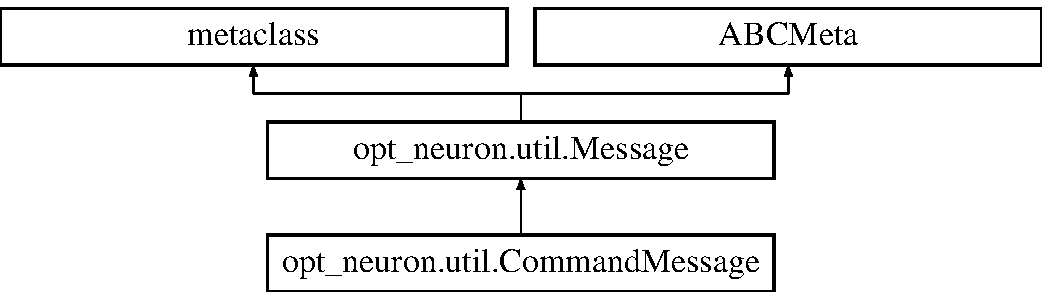
\includegraphics[height=3.000000cm]{classopt__neuron_1_1util_1_1CommandMessage}
\end{center}
\end{figure}
\subsection*{Public Member Functions}
\begin{DoxyCompactItemize}
\item 
\hypertarget{classopt__neuron_1_1util_1_1CommandMessage_ac47ba4ba7dae61dc3a6c02c0d3f99c6c}{}def {\bfseries \+\_\+\+\_\+init\+\_\+\+\_\+}\label{classopt__neuron_1_1util_1_1CommandMessage_ac47ba4ba7dae61dc3a6c02c0d3f99c6c}

\item 
\hypertarget{classopt__neuron_1_1util_1_1CommandMessage_a012e016e20502d0b4b1eb652378192c7}{}def {\bfseries type} (self)\label{classopt__neuron_1_1util_1_1CommandMessage_a012e016e20502d0b4b1eb652378192c7}

\end{DoxyCompactItemize}
\subsection*{Additional Inherited Members}


The documentation for this class was generated from the following file\+:\begin{DoxyCompactItemize}
\item 
opt\+\_\+neuron/util.\+py\end{DoxyCompactItemize}

\hypertarget{classopt__neuron_1_1util_1_1Message}{}\section{opt\+\_\+neuron.\+util.\+Message Class Reference}
\label{classopt__neuron_1_1util_1_1Message}\index{opt\+\_\+neuron.\+util.\+Message@{opt\+\_\+neuron.\+util.\+Message}}
Inheritance diagram for opt\+\_\+neuron.\+util.\+Message\+:\begin{figure}[H]
\begin{center}
\leavevmode
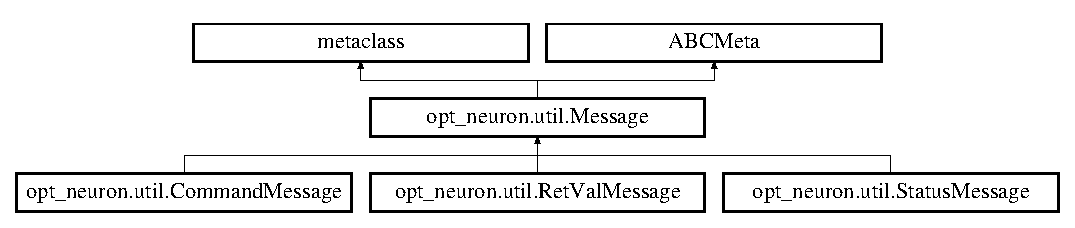
\includegraphics[height=2.616822cm]{classopt__neuron_1_1util_1_1Message}
\end{center}
\end{figure}
\subsection*{Public Member Functions}
\begin{DoxyCompactItemize}
\item 
\hypertarget{classopt__neuron_1_1util_1_1Message_a376cf143778d5ed3cefd3c7dcc1fbc40}{}def {\bfseries \+\_\+\+\_\+init\+\_\+\+\_\+}\label{classopt__neuron_1_1util_1_1Message_a376cf143778d5ed3cefd3c7dcc1fbc40}

\item 
def \hyperlink{classopt__neuron_1_1util_1_1Message_ae0ff9396bfe89407875ce4892e049993}{type} (self)
\item 
\hypertarget{classopt__neuron_1_1util_1_1Message_afd67ea4cba1d4fbab576f0390fcdf26c}{}def {\bfseries id} (self)\label{classopt__neuron_1_1util_1_1Message_afd67ea4cba1d4fbab576f0390fcdf26c}

\item 
\hypertarget{classopt__neuron_1_1util_1_1Message_a14ba24a31153719e086c62c09a2b595d}{}def {\bfseries priority} (self)\label{classopt__neuron_1_1util_1_1Message_a14ba24a31153719e086c62c09a2b595d}

\item 
\hypertarget{classopt__neuron_1_1util_1_1Message_ace24c823ca2e199b6a5a4f76a8d8e8cf}{}def {\bfseries content} (self)\label{classopt__neuron_1_1util_1_1Message_ace24c823ca2e199b6a5a4f76a8d8e8cf}

\item 
\hypertarget{classopt__neuron_1_1util_1_1Message_aa5d6f183c7fe764bb9fedd50efd722be}{}def {\bfseries \+\_\+\+\_\+repr\+\_\+\+\_\+} (self)\label{classopt__neuron_1_1util_1_1Message_aa5d6f183c7fe764bb9fedd50efd722be}

\item 
\hypertarget{classopt__neuron_1_1util_1_1Message_a08b095ada3d0f88ce43b444d975ec118}{}def {\bfseries \+\_\+\+\_\+eq\+\_\+\+\_\+} (self, other)\label{classopt__neuron_1_1util_1_1Message_a08b095ada3d0f88ce43b444d975ec118}

\item 
\hypertarget{classopt__neuron_1_1util_1_1Message_a87492c040e73da9af2b600b47ce2ffa0}{}def {\bfseries \+\_\+\+\_\+lt\+\_\+\+\_\+} (self, other)\label{classopt__neuron_1_1util_1_1Message_a87492c040e73da9af2b600b47ce2ffa0}

\end{DoxyCompactItemize}
\subsection*{Public Attributes}
\begin{DoxyCompactItemize}
\item 
\hypertarget{classopt__neuron_1_1util_1_1Message_af95a73f8917821dd2913edfc88047866}{}{\bfseries content}\label{classopt__neuron_1_1util_1_1Message_af95a73f8917821dd2913edfc88047866}

\item 
\hypertarget{classopt__neuron_1_1util_1_1Message_ac0bd62aa1bb7068ef6242dcb39837292}{}{\bfseries priority}\label{classopt__neuron_1_1util_1_1Message_ac0bd62aa1bb7068ef6242dcb39837292}

\item 
\hypertarget{classopt__neuron_1_1util_1_1Message_a1d45ea876af6ba9c5b3c92f10c768c08}{}{\bfseries type}\label{classopt__neuron_1_1util_1_1Message_a1d45ea876af6ba9c5b3c92f10c768c08}

\end{DoxyCompactItemize}


\subsection{Detailed Description}
\begin{DoxyVerb}Message encapsulates a message.
A message has got a type (subclassed), an id, a priority and \
content, of course.
\end{DoxyVerb}
 

\subsection{Member Function Documentation}
\hypertarget{classopt__neuron_1_1util_1_1Message_ae0ff9396bfe89407875ce4892e049993}{}\index{opt\+\_\+neuron\+::util\+::\+Message@{opt\+\_\+neuron\+::util\+::\+Message}!type@{type}}
\index{type@{type}!opt\+\_\+neuron\+::util\+::\+Message@{opt\+\_\+neuron\+::util\+::\+Message}}
\subsubsection[{type(self)}]{\setlength{\rightskip}{0pt plus 5cm}def opt\+\_\+neuron.\+util.\+Message.\+type (
\begin{DoxyParamCaption}
\item[{}]{self}
\end{DoxyParamCaption}
)}\label{classopt__neuron_1_1util_1_1Message_ae0ff9396bfe89407875ce4892e049993}
\begin{DoxyVerb}To be overwritten in subclasses. Should return a MessageType object.
\end{DoxyVerb}
 

The documentation for this class was generated from the following file\+:\begin{DoxyCompactItemize}
\item 
opt\+\_\+neuron/util.\+py\end{DoxyCompactItemize}

\hypertarget{classopt__neuron_1_1util_1_1MessageQueue}{}\section{opt\+\_\+neuron.\+util.\+Message\+Queue Class Reference}
\label{classopt__neuron_1_1util_1_1MessageQueue}\index{opt\+\_\+neuron.\+util.\+Message\+Queue@{opt\+\_\+neuron.\+util.\+Message\+Queue}}
Inheritance diagram for opt\+\_\+neuron.\+util.\+Message\+Queue\+:\begin{figure}[H]
\begin{center}
\leavevmode
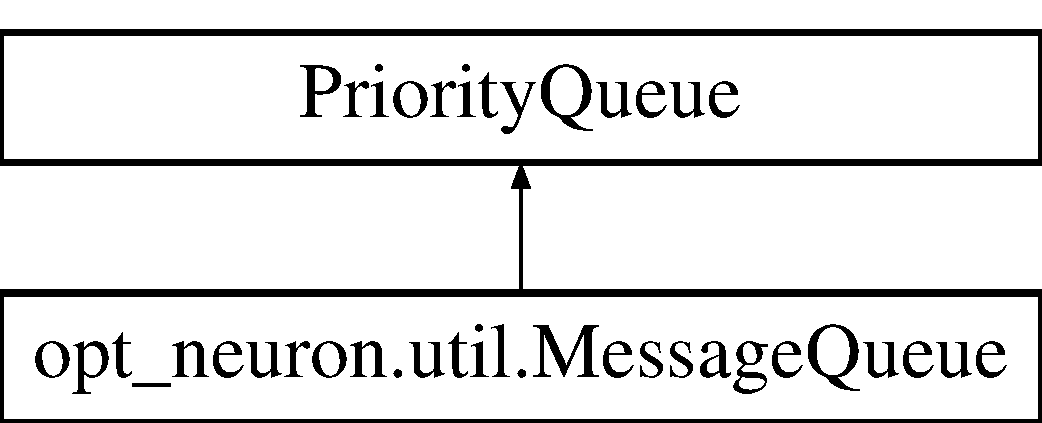
\includegraphics[height=2.000000cm]{classopt__neuron_1_1util_1_1MessageQueue}
\end{center}
\end{figure}
\subsection*{Public Member Functions}
\begin{DoxyCompactItemize}
\item 
\hypertarget{classopt__neuron_1_1util_1_1MessageQueue_aefdcf179ba76aa2d5bea24b5667ed212}{}def {\bfseries put}\label{classopt__neuron_1_1util_1_1MessageQueue_aefdcf179ba76aa2d5bea24b5667ed212}

\item 
\hypertarget{classopt__neuron_1_1util_1_1MessageQueue_a8877bd018f1eb539bb70d1a4fcf59938}{}def {\bfseries get}\label{classopt__neuron_1_1util_1_1MessageQueue_a8877bd018f1eb539bb70d1a4fcf59938}

\end{DoxyCompactItemize}


\subsection{Detailed Description}
\begin{DoxyVerb}Adaption of the PriorityQueue class.
Only objects of type Message can be put in this queue as the name already suggests.
Every sent message will be logged (Level: DEBUG)
\end{DoxyVerb}
 

The documentation for this class was generated from the following file\+:\begin{DoxyCompactItemize}
\item 
opt\+\_\+neuron/util.\+py\end{DoxyCompactItemize}

\hypertarget{classopt__neuron_1_1util_1_1MessageType}{}\section{opt\+\_\+neuron.\+util.\+Message\+Type Class Reference}
\label{classopt__neuron_1_1util_1_1MessageType}\index{opt\+\_\+neuron.\+util.\+Message\+Type@{opt\+\_\+neuron.\+util.\+Message\+Type}}
Inheritance diagram for opt\+\_\+neuron.\+util.\+Message\+Type\+:\begin{figure}[H]
\begin{center}
\leavevmode
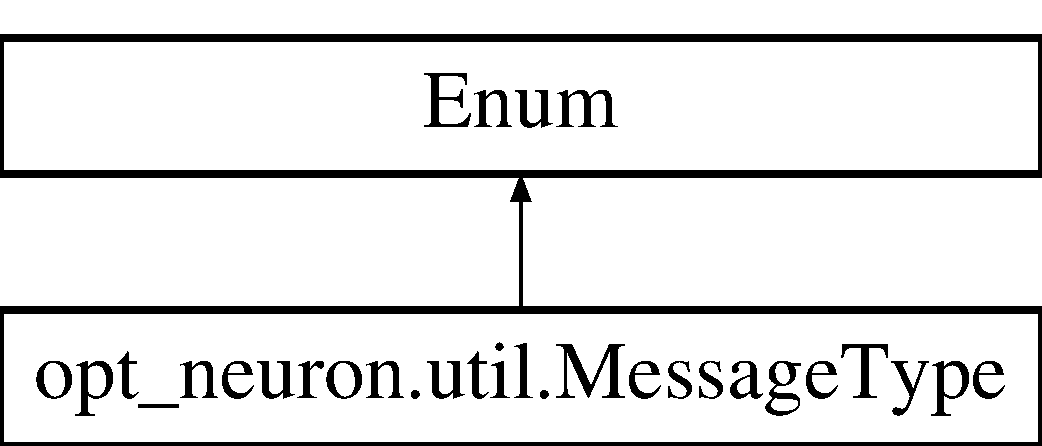
\includegraphics[height=2.000000cm]{classopt__neuron_1_1util_1_1MessageType}
\end{center}
\end{figure}
\subsection*{Static Public Attributes}
\begin{DoxyCompactItemize}
\item 
\hypertarget{classopt__neuron_1_1util_1_1MessageType_a3fc09d8b0442815791b847fe240e0665}{}int {\bfseries S\+T\+A\+T\+U\+S} = 1\label{classopt__neuron_1_1util_1_1MessageType_a3fc09d8b0442815791b847fe240e0665}

\item 
\hypertarget{classopt__neuron_1_1util_1_1MessageType_a8400073e1604c2b134cb71d4803eba24}{}int {\bfseries C\+O\+M\+M\+A\+N\+D} = 2\label{classopt__neuron_1_1util_1_1MessageType_a8400073e1604c2b134cb71d4803eba24}

\item 
\hypertarget{classopt__neuron_1_1util_1_1MessageType_a59133ead95d5110d60c483c5151e728f}{}int {\bfseries R\+E\+T\+V\+A\+L} = 3\label{classopt__neuron_1_1util_1_1MessageType_a59133ead95d5110d60c483c5151e728f}

\end{DoxyCompactItemize}


The documentation for this class was generated from the following file\+:\begin{DoxyCompactItemize}
\item 
opt\+\_\+neuron/util.\+py\end{DoxyCompactItemize}

\hypertarget{classopt__neuron_1_1util_1_1RetValMessage}{}\section{opt\+\_\+neuron.\+util.\+Ret\+Val\+Message Class Reference}
\label{classopt__neuron_1_1util_1_1RetValMessage}\index{opt\+\_\+neuron.\+util.\+Ret\+Val\+Message@{opt\+\_\+neuron.\+util.\+Ret\+Val\+Message}}
Inheritance diagram for opt\+\_\+neuron.\+util.\+Ret\+Val\+Message\+:\begin{figure}[H]
\begin{center}
\leavevmode
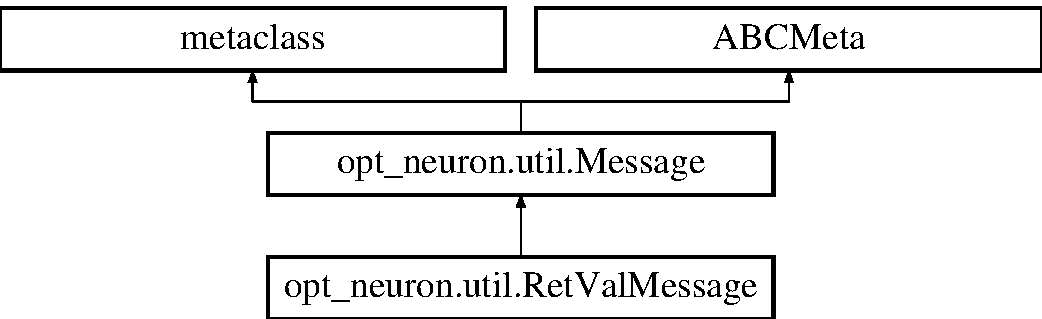
\includegraphics[height=3.000000cm]{classopt__neuron_1_1util_1_1RetValMessage}
\end{center}
\end{figure}
\subsection*{Public Member Functions}
\begin{DoxyCompactItemize}
\item 
\hypertarget{classopt__neuron_1_1util_1_1RetValMessage_aeb8d852b9b862fde597ce0a92c2146a7}{}def {\bfseries \+\_\+\+\_\+init\+\_\+\+\_\+}\label{classopt__neuron_1_1util_1_1RetValMessage_aeb8d852b9b862fde597ce0a92c2146a7}

\item 
\hypertarget{classopt__neuron_1_1util_1_1RetValMessage_afdb43ad240de3ca349c0e0c7a1ae8617}{}def {\bfseries appendix} (self)\label{classopt__neuron_1_1util_1_1RetValMessage_afdb43ad240de3ca349c0e0c7a1ae8617}

\item 
\hypertarget{classopt__neuron_1_1util_1_1RetValMessage_a3ca5b6a7b898f583f15009dd94727a85}{}def {\bfseries cmd\+\_\+id} (self)\label{classopt__neuron_1_1util_1_1RetValMessage_a3ca5b6a7b898f583f15009dd94727a85}

\item 
\hypertarget{classopt__neuron_1_1util_1_1RetValMessage_ab0ca46a68582f092def08437ee57c506}{}def {\bfseries type} (self)\label{classopt__neuron_1_1util_1_1RetValMessage_ab0ca46a68582f092def08437ee57c506}

\end{DoxyCompactItemize}
\subsection*{Additional Inherited Members}


The documentation for this class was generated from the following file\+:\begin{DoxyCompactItemize}
\item 
opt\+\_\+neuron/util.\+py\end{DoxyCompactItemize}

\hypertarget{classopt__neuron_1_1util_1_1StatusMessage}{}\section{opt\+\_\+neuron.\+util.\+Status\+Message Class Reference}
\label{classopt__neuron_1_1util_1_1StatusMessage}\index{opt\+\_\+neuron.\+util.\+Status\+Message@{opt\+\_\+neuron.\+util.\+Status\+Message}}
Inheritance diagram for opt\+\_\+neuron.\+util.\+Status\+Message\+:\begin{figure}[H]
\begin{center}
\leavevmode
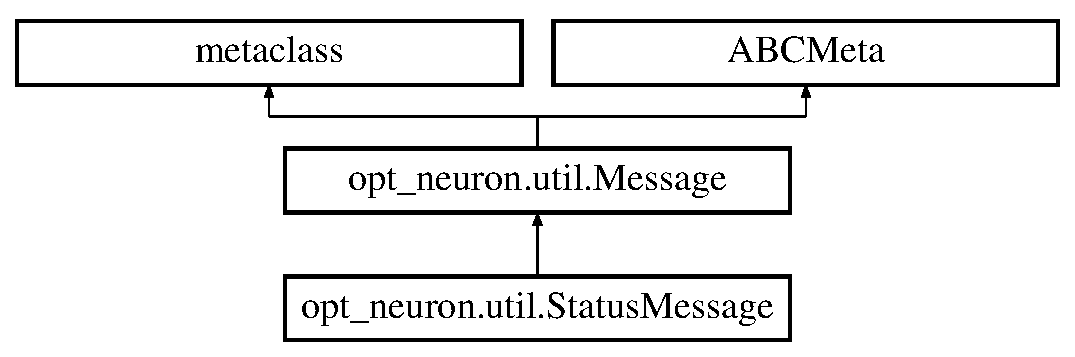
\includegraphics[height=3.000000cm]{classopt__neuron_1_1util_1_1StatusMessage}
\end{center}
\end{figure}
\subsection*{Public Member Functions}
\begin{DoxyCompactItemize}
\item 
\hypertarget{classopt__neuron_1_1util_1_1StatusMessage_abd4de006fbca5082fba18c7f5a4108b6}{}def {\bfseries type} (self)\label{classopt__neuron_1_1util_1_1StatusMessage_abd4de006fbca5082fba18c7f5a4108b6}

\end{DoxyCompactItemize}
\subsection*{Additional Inherited Members}


The documentation for this class was generated from the following file\+:\begin{DoxyCompactItemize}
\item 
opt\+\_\+neuron/util.\+py\end{DoxyCompactItemize}

%--- End generated contents ---

% Index
\backmatter
\newpage
\phantomsection
\clearemptydoublepage
\addcontentsline{toc}{chapter}{Index}
\printindex

\end{document}
